\setlength{\parindent}{0pt}
\setlength{\parskip}{5pt}

\noindent
\begin{minipage}[t]{120pt}
    \vspace*{110pt}
    \noindent
    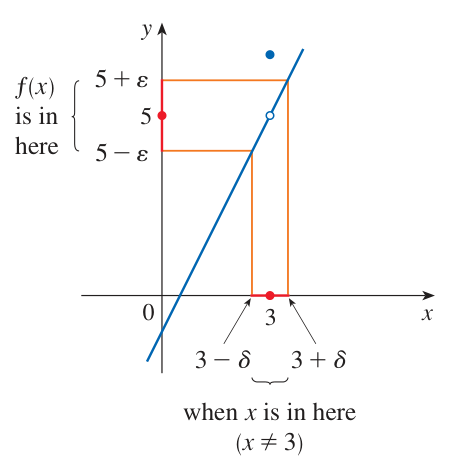
\includegraphics[width=\linewidth]{images/p0141_fig1.png}

    \vspace{4pt}
    \noindent
    {\fontsize{8.5pt}{10pt}\selectfont\textbf{\textsf{HÌNH 1}}}

    \vspace{24pt}
    \noindent
    {\fontsize{8pt}{10.5pt}\selectfont\color{stewartdark}\raggedright
    Theo truyền thống, người ta thường dùng các chữ cái Hy Lạp $\varepsilon$ và $\delta$ trong định nghĩa chính xác của giới hạn.\par}
\end{minipage}%
\hspace{18pt}%
\begin{minipage}[t]{366pt}
    Các số $0{,}1$; $0{,}01$ và $0{,}001$ mà chúng ta đã xem xét là những \emph{dung sai sai số} mà ta có thể cho phép. Để $5$ là giới hạn chính xác của $f(x)$ khi $x$ tiến dần đến $3$, chúng ta không chỉ cần làm cho hiệu giữa $f(x)$ và $5$ nhỏ hơn mỗi số trong ba số nói trên; mà ta phải có thể làm cho nó nhỏ hơn \emph{bất kỳ} số dương nào. Và bằng lập luận tương tự, chúng ta hoàn toàn có thể làm được! Nếu ta viết $\varepsilon$ (chữ cái Hy Lạp epsilon) để biểu thị một số dương tùy ý, thì tương tự như trước, ta thấy rằng

    \vspace{2pt}
    \noindent
    \makebox[\linewidth]{%
      \makebox[0pt][l]{\hspace*{10pt}\stewartboxnum{1}}%
      \hfill
      $\displaystyle |f(x) - 5| < \varepsilon \qquad \text{nếu} \qquad 0 < |x - 3| < \delta = \frac{\varepsilon}{2}$%
      \hfill
    }
    \vspace{2pt}

    Đây là một cách nói chính xác rằng $f(x)$ ở gần $5$ khi $x$ ở gần $3$ bởi vì (1) khẳng định rằng ta có thể làm cho các giá trị của $f(x)$ nằm trong khoảng cách tùy ý $\varepsilon$ so với $5$ bằng cách giới hạn các giá trị của $x$ nằm trong khoảng cách $\varepsilon/2$ so với $3$ (nhưng $x \neq 3$).

    Lưu ý rằng (1) có thể được viết lại như sau:
    {\setlength{\abovedisplayskip}{4pt}\setlength{\belowdisplayskip}{4pt}
    \[
    \text{nếu} \quad 3 - \delta < x < 3 + \delta \quad (x \neq 3) \qquad \text{thì} \qquad 5 - \varepsilon < f(x) < 5 + \varepsilon
    \]}
    và điều này được minh họa trong Hình~1. Bằng cách lấy các giá trị của $x$ ($x \neq 3$) nằm trong khoảng $(3 - \delta, 3 + \delta)$, ta có thể làm cho các giá trị của $f(x)$ nằm trong khoảng $(5 - \varepsilon, 5 + \varepsilon)$.

    Sử dụng (1) làm mẫu, chúng ta đưa ra định nghĩa chính xác về giới hạn.

    \vspace{1pt}
    \begin{tcolorbox}[
      colback=white,
      colframe=stewartred,
      boxrule=0.9pt,
      sharp corners,
      boxsep=0pt,
      left=8pt, right=8pt,
      top=7pt, bottom=7pt
    ]
    \setlength{\abovedisplayskip}{4.5pt}
    \setlength{\belowdisplayskip}{4.5pt}
    \noindent
    \stewartboxnum{2}\hspace{6pt}{\bfseries\sffamily\fontsize{10pt}{12pt}\selectfont\color{stewartred}Định nghĩa chính xác của giới hạn}\quad
    Giả sử $f$ là một hàm số xác định trên một khoảng mở nào đó chứa số $a$, ngoại trừ có thể tại chính điểm $a$. Khi đó ta nói rằng \textbf{giới hạn của $\boldsymbol{f(x)}$ khi $\boldsymbol{x}$ tiến tới $\boldsymbol{a}$ là $\boldsymbol{L}$}, và viết
    \[
    \lim_{x \to a} f(x) = L
    \]
    nếu với mỗi số $\varepsilon > 0$ đều tồn tại một số $\delta > 0$ sao cho
    \[
    \text{nếu} \quad 0 < |x - a| < \delta \qquad \text{thì} \qquad |f(x) - L| < \varepsilon
    \]
    \end{tcolorbox}
    \vspace{1pt}

    Vì $|x - a|$ là khoảng cách từ $x$ đến $a$ và $|f(x) - L|$ là khoảng cách từ $f(x)$ đến $L$, đồng thời do $\varepsilon$ có thể nhỏ tùy ý, nên định nghĩa về giới hạn có thể được diễn đạt bằng lời như sau:

    \begin{stewartdesc}
    $\lim\limits_{x \to a} f(x) = L$ có nghĩa là khoảng cách giữa $f(x)$ và $L$ có thể được làm cho nhỏ tùy ý bằng cách yêu cầu khoảng cách từ $x$ đến $a$ phải đủ nhỏ (nhưng khác $0$).
    \end{stewartdesc}

    Nói cách khác,

    \begin{stewartdesc}
    $\lim\limits_{x \to a} f(x) = L$ có nghĩa là các giá trị của $f(x)$ có thể được làm cho gần $L$ bao nhiêu tùy ý bằng cách yêu cầu $x$ phải đủ gần $a$ (nhưng không bằng $a$).
    \end{stewartdesc}

    Chúng ta cũng có thể phát biểu lại Định nghĩa~2 theo ngôn ngữ các khoảng bằng cách nhận xét rằng bất đẳng thức $|x - a| < \delta$ tương đương với $-\delta < x - a < \delta$, từ đó có thể viết lại thành $a - \delta < x < a + \delta$. Ngoài ra, $0 < |x - a|$ đúng khi và chỉ khi $x - a \neq 0$, tức là $x \neq a$. Tương tự, bất đẳng thức $|f(x) - L| < \varepsilon$ tương đương với cặp bất đẳng thức $L - \varepsilon < f(x) < L + \varepsilon$. Do đó, theo ngôn ngữ các khoảng, Định nghĩa~2 có thể được phát biểu như sau:

    \begin{stewartdesc}
    $\lim\limits_{x \to a} f(x) = L$ có nghĩa là với mọi số $\varepsilon > 0$ (cho dù $\varepsilon$ có nhỏ đến đâu), ta luôn tìm được một số $\delta > 0$ sao cho nếu $x$ nằm trong khoảng mở $(a - \delta, a + \delta)$ và $x \neq a$, thì $f(x)$ nằm trong khoảng mở $(L - \varepsilon, L + \varepsilon)$.
    \end{stewartdesc}
\end{minipage}
